När Matlabb startas möts man av MatLabbs hjärta, Sök-vyn. Det är här
användaren söker efter och öppnar recept. Det finns två sätt att söka
efter recept i MatLabb, Titelsök och Filtersök.

\begin{figure}[h]
        \centering 
        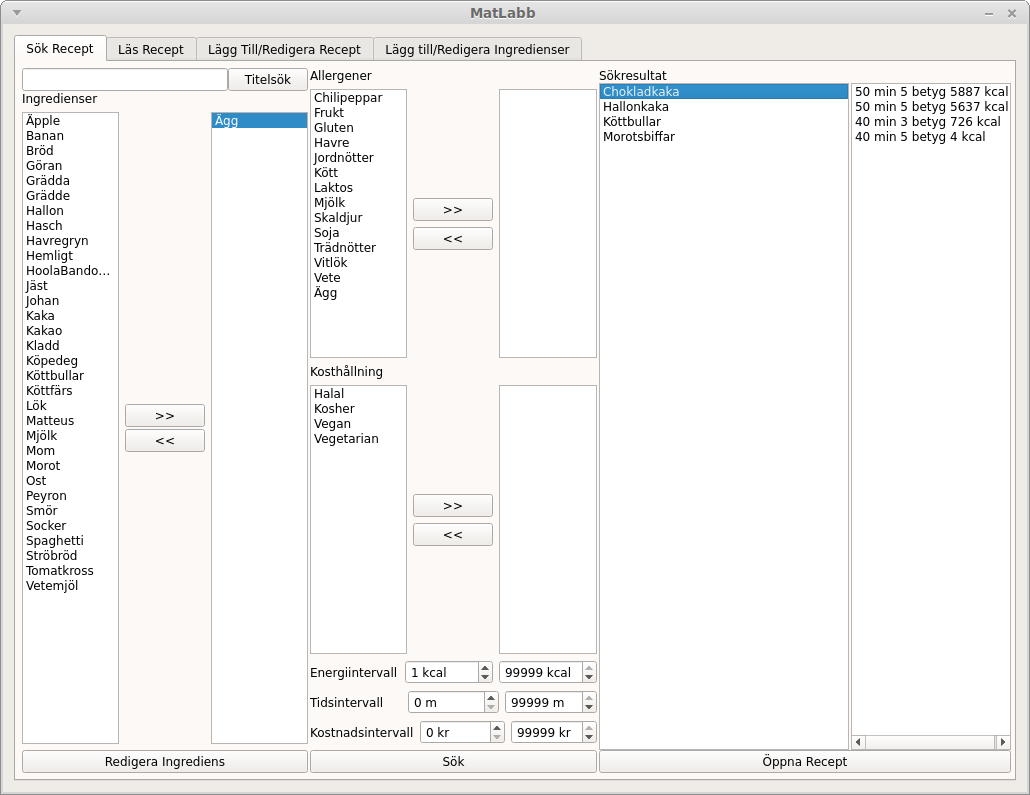
\includegraphics[scale=0.44]{sok_recept.png} 
        \caption{Sökvyn} 
        \label{fig:sokvyn}
\end{figure}


\subsection{Titelsökning}
Vet man redan vilket recept man är ute efter kan det enkelt och snabbt
hittas med hjälp av titelsökfunktionen. Receptets namn matas in i
titelsökrutan och hittas med \verb+Titelsök+-knappen och kan sedan öppnas
med knappen \verb+Öppna+. Medans detta räcker för många kan även den
avancerade användaren istället filtrera sina sökningar.

\subsection{Filtersökning}

Matlabb har ett flertal avancerade filtreringsmekanismer, varav den
mest centrala är ingrediensfiltrering. Ingrediensfiltret finns till
vänster i sök-vyn märkt Ingredienser. För att inkludera en ingrediens
i listan markeras den och flyttas till Sök-listan med hjälp av \verb+>>+
knappen. Vill man ta bort en ingrediens från sök-listan görs detta med
hjälp av \verb+<<+ knappen.

Till höger om ingredienslistan ses två liknande listor. Allergier samt
kosthållning som används för att filtrera bort recept innehållande en
viss allergen eller ifall man vill exkludera recept av etiska,
religiösa eller andra skäl. Dessa fungerar på precis samma sätt som för
ingrediensfiltrering.

Under kosthållningslistan finns filtren för energiinnehåll tidsåtgång
och portionskostnad. Filtreringen görs genom att markera fälten brevid respektive etikett. Därefter skriver man in i det vänstra fältet en min-gräns och i fältet till höger en maxgräns. Filtersökningen kommer inte visa resultat som ligger utanför dessa intervall.

När filtreringsinställningarna är färdiga slutförs sökningen genom att
knappen \verb+Sök+ trycks in och recepten dyker upp i listan till
höger. För att öppna ett recept markeras dess namn och när
knappen \verb+öppna+ trycks in skickas man vidare till recept-vyn.

I sökvyn finns funktionalitet för att redigera ingredienser. En ingrediens kan markeras på samma sätt som om man skulle söka på det, fast istället för att klicka på \verb+>>+, klickar man på knappen \verb+Redigera Ingrediens+. Ingrediensen öppnas då i vyn. Se kapitel \ref{adding} för vidare information om att lägga till eller redigera ingredienser. 
